We saw in Section~\ref{sec:threed_sr_as_generalbinary} that an instance $(N, V)$ of 3DR-AS may not contain a stable matching, and the associated decision problem is $\NP$-complete, even when valuations are binary. It follows that the decision problem for ternary valuations, i.e.\ $v_{\alpha_i}(\alpha_j) \in \{ 0, 1, 2 \}$ for each $\alpha_i, \alpha_j \in N$ is also $\NP$-complete. In contrast we saw in Section~\ref{sec:threed_sr_as_symmetricbinary} that when valuations are binary and symmetric a stable matching always exists and can be found in polynomial time. It is natural to ask if this polynomial-time solvability also holds in the more general case of ternary and symmetric valuations. We answer this question in the negative (assuming $\P=\NP$), and show that deciding if a given instance of 3DR-AS contains a stable matching is $\NP$-complete, even when valuations are ternary and symmetric. We remark that a result of Deineko and Woeginger \cite{DEINEKO20131837} for \emph{Geometric 3D-SR} (see Chapter~\ref{c:lit_review}) implies a weaker version of our result, namely that if valuations are symmetric (but not necessarily ternary) then deciding if a given instance of 3DR-AS contains a stable matching is $\NP$-complete, even when valuations are ternary and symmetric.

% We define 3DR as the restriction of 3D-SR-AS in which valuations are ternary and symmetric. Like 3D-SR-AS, the decision version of 3D-SR-SAS-TER belongs to the class $\NP$. 

We present a polynomial-time reduction from Partition into Triangles (PIT, Problem~\ref{prob:pit}), which is similar to the reduction that we presented in Section~\ref{sec:threed_sr_as_generalbinary} for the analogous decision problem involving preferences that are binary but not necessarily symmetric. The main difference is in the design of the gadgets. Instead of ``pentagadgets'' we introduce a number of ``octogadgets''. Nevertheless, the purpose of the octogadgets is the same as the pentagadgets in the previous reduction and the proof follows the same structure as before.

The reduction, illustrated in Figure~\ref{fig:threed_sr_as_ternary_symmetric_reduction}, is as follows. Since valuations are symmetric in $(N, V)$, we shall usually specify valuations in one direction only. For example, instead of writing ``let $v_{\alpha_i}(\alpha_j)=v_{\alpha_j}(\alpha_i)=1$'' we write ``let $v_{\alpha_i}(\alpha_j)=1$''. Unless otherwise specified assume that $v_{\alpha_i}(\alpha_j)=0$ for any $\alpha_i, \alpha_j \in N$. To simplify the description of the valuations in the reduction, in this section we write $i \myoplus y$ to denote $((i + y - 1) \bmod 8) + 1$.

For each $i$ where $1\leq i \leq 3q$ construct three agents labelled $a_{2i}$, $a_{2i-1}$, and $b_i$. Let $v_{a_{2i}}(a_{2i-1}) = v_{b_i}(a_{2i}) = v_{b_i}(a_{2i-1}) = 1$. For each $w_i, w_j \in W$ let $v_{b_i}(b_j)=1$ if $\{ w_i, w_j \} \in E$ and $0$ otherwise. Next, for each $r$ where $1 \leq r \leq 6q$ construct a set of eight agents $H_r = \{ h_r^1, h_r^2, \dots, h_r^8 \}$, which we refer to as the \emph{$h\textsuperscript{th}$ octogadget}. For each $i$ and $j$ where $1\leq i, j \leq 8$ let $v_{h_r^i}(h_r^j) = 2$ if both $i$ is odd and $j = i \myoplus 1$ otherwise $1$.
This completes the construction of $(N, V)$. Note that $|N| = 57q$.

\begin{figure}
    \centering
    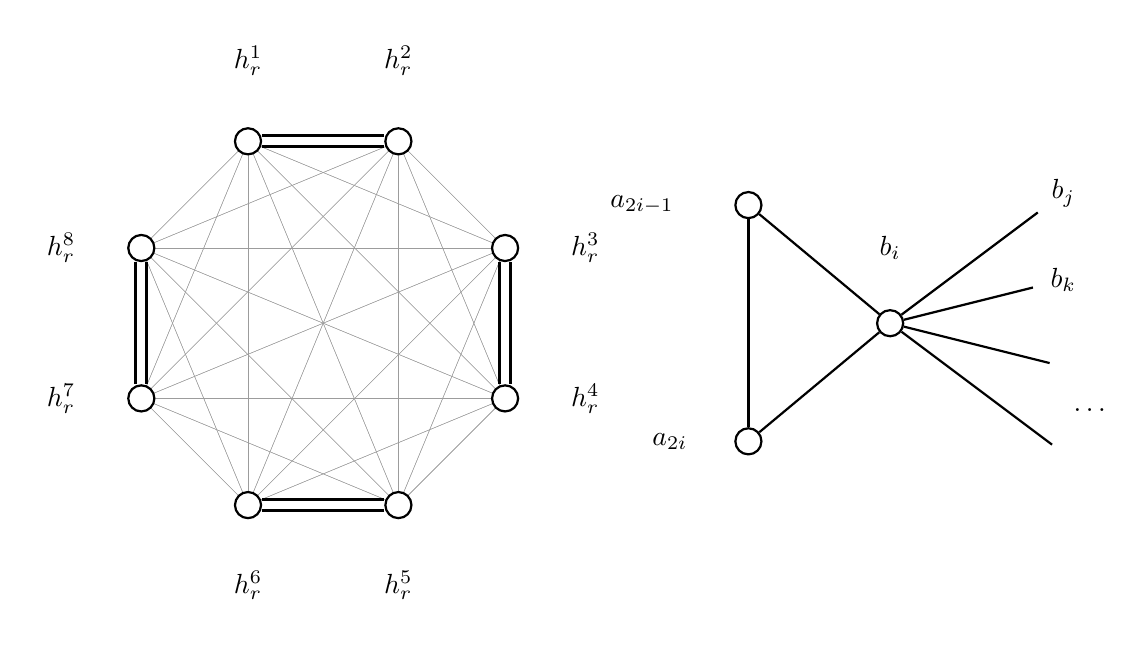
\begin{tikzpicture}
% \draw[help lines] (0,0) grid (12,6);
\begin{scope}[every node/.style={circle,thick,draw,minimum size=2.4mm}, scale=1.0]
    % \node[draw=none, align=center] (Pc) at (2.4,-0.5) {octogadget $H_r$ for some $1\leq r \leq 6q$};
    
    \def\hscale{0.5}
    
    % this one the angles are the same
    % \begin{scope}[shift={(3.0, 3.0)}]
    % \node[draw=none] (hr1i) at (\hscale*0 ,\hscale*-5) {};
    % \node[draw=none] (hr2i) at (\hscale*-3,\hscale*-4) {};
    % \node[draw=none] (hr3i) at (\hscale*-5,\hscale*-2) {};
    % \node[draw=none] (hr4i) at (\hscale*-5,\hscale*1) {};
    % \node[draw=none] (hr5i) at (\hscale*-4,\hscale*3) {};
    % \node[draw=none] (hr6i) at (\hscale*-1,\hscale*5) {};
    % \node[draw=none] (hr7i) at (\hscale*1,\hscale*5) {};
    % \node[draw=none] (hr8i) at (\hscale*4,\hscale*3) {};
    % \node[draw=none] (hr9i) at (\hscale*5,\hscale*1) {};
    % \node[draw=none] (hr10i) at (\hscale*5,\hscale*-2) {};
    % \node[draw=none] (hr11i) at (\hscale*3,\hscale*-4) {};
    % \end{scope}
    
    % this one is a 12-gon with the two at the bottom merged
    \begin{scope}[shift={(2.8, 3.0)}]
    % http://www.rotaryspin.com/markb/courses/projects/polygon.html
    \node[draw=none] (hr3i) at (\hscale*4.62,\hscale*1.91) {};
    \node[draw=none] (hr2i) at (\hscale*1.91,\hscale*4.62) {};
    \node[draw=none] (hr1i) at (\hscale*-1.91,\hscale*4.62) {};
    \node[draw=none] (hr8i) at (\hscale*-4.62,\hscale*1.91) {};
    \node[draw=none] (hr7i) at (\hscale*-4.62,\hscale*-1.91) {};
    \node[draw=none] (hr6i) at (\hscale*-1.91,\hscale*-4.62) {};
    \node[draw=none] (hr5i) at (\hscale*1.91,\hscale*-4.62) {};
    \node[draw=none] (hr4i) at (\hscale*4.62,\hscale*-1.91) {};
    \end{scope}
    
    \def\hlabeldist{0.4cm}
    
    \node[label={[label distance=\hlabeldist]90:$b_i$}] (bi) at (10,3) {};
    \node[label={[label distance=\hlabeldist]180:$a_{2i}$}] (ai1) at (8.2,1.5) {};
    \node[label={[label distance=\hlabeldist+0.19cm]180:$a_{2i-1}$}] (ai2) at (8.2,4.5) {};
    \node[draw=none] (bk1) at (12.2,1.35) {};
    \node[draw=none] (bk2) at (12.2,2.45) {};
    \node[draw=none] (bkdots) at (12.5,1.9) {\hspace{2pt}$\dots$};
    \node[draw=none] (bj) at (12.2,3.55) {$b_k$};
    \node[draw=none] (bk) at (12.2,4.65) {$b_j$};
    % \node[draw=none, text width=6cm, align=center] (aic) at (10.2,0.-0.4) {for each $1\leq i\leq 3q$ where $N(w_i)=\{ w_j, w_k, \dots \}$};
\end{scope}
\begin{scope}
    \foreach \from in {hr1i, hr2i, hr3i, hr4i, hr5i, hr6i, hr7i, hr8i}{
        \foreach \to in {hr1i, hr2i, hr3i, hr4i, hr5i, hr6i, hr7i, hr8i}
            \draw[line width=0.05mm,color=black!39] (\from.center) -- (\to.center);
    }
    
    % \fill [black!10] (hr1i.center) -- (hr2i.center) -- (hr3i.center) -- (hr4i.center) -- (hr5i.center) -- (hr6i.center) -- (hr7i.center) -- (hr8i.center) -- (hr9i.center) -- (hr10i.center) -- (hr11i.center) -- cycle;
    
    \foreach \from/\to in {hr1i/hr2i, hr3i/hr4i, hr5i/hr6i, hr7i/hr8i}
        \draw [black, double=white, line width = 1pt, double distance = 3pt ] (\from) -- (\to);
    
    
    % \foreach \from/\to in {pr2/pr1, pr3/pr2, pr4/pr3, pr5/pr4, pr1/pr5}
    %     \path [thick, -<--] (\from) -- (\to);
    % \foreach \from/\to in {pr1/pr3, pr3/pr5, pr5/pr2, pr2/pr4, pr4/pr1}
        % \draw [thick] (\from) -- (\to);
    % TRIANGLE
     \foreach \from/\to in {bi/bj, bi/bk, bi/bk1, bi/bk2}
        \draw [thick] (\from) -- (\to);
    \foreach \from/\to in {bi/ai1, ai1/ai2, ai2/bi}
        \draw [thick] (\from) -- (\to);
    \foreach \from/\to in {ai1/bi, ai2/ai1, bi/ai2}
        \path [thick] (\from) -- (\to);
\end{scope}
\begin{scope}[every node/.style={circle,thick,draw,minimum size=2.4mm, fill=white}, scale=1.0]
    \def\hlabeldist{0.4cm}
    
    \node[thick, circle, label={[label distance=\hlabeldist]90:$h_r^1$}] (hr1) at (hr1i) {};
    \node[thick, circle, label={[label distance=\hlabeldist]90:$h_r^2$}] (hr2) at (hr2i) {};
    \node[thick, circle, label={[label distance=\hlabeldist]0:$h_r^3$}] (hr3) at (hr3i) {};
    \node[thick, circle, label={[label distance=\hlabeldist]0:$h_r^4$}] (hr4) at (hr4i) {};
    \node[thick, circle, label={[label distance=\hlabeldist]270:$h_r^5$}] (hr5) at (hr5i) {};
    \node[thick, circle, label={[label distance=\hlabeldist]270:$h_r^6$}] (hr6) at (hr6i) {};
    \node[thick, circle, label={[label distance=\hlabeldist]180:$h_r^7$}] (hr7) at (hr7i) {};
    \node[thick, circle, label={[label distance=\hlabeldist]180:$h_r^8$}] (hr8) at (hr8i) {};
\end{scope}
\end{tikzpicture}

    
    
    
    
    
    
    
    

%%%%%%%%%%%%%%%%%%%%%%%%%%%%%%%%%%%%%%%%%%%%%%%%%%%%%%%%%%%%%%%%%%%%%%
%%%%%%%%%%%%%%%%%%%%%%%%%%%%%%%%%%%%%%%%%%%%%%%%%%%%%%%%%%%%%%%%%%%%%%
%%%%%%%%%%%%%%%%%%%%%%%%%%%%%%%%%%%%%%%%%%%%%%%%%%%%%%%%%%%%%%%%%%%%%%


% OLD VERSION with labels inside nodes


% \begin{tikzpicture}
% % \draw[help lines] (0,0) grid (12,6);
% \begin{scope}[every node/.style={circle,thick,draw,inner sep=0.8mm,minimum size=1.6mm}, scale=1.0]
%     % \node (A) at (6,0) {$.$};
%     % \node (B) at (6,6) {$.$};
%     \node[draw=none, align=center] (Pc) at (3,-0.6) {hendecagadget $H_r$ for some $1\leq r \leq 6q$};
    
%     \def\hscale{0.55}
    
%     % this one the angles are the same
%     % \begin{scope}[shift={(3.0, 3.0)}]
%     % % https://www.mathopenref.com/coordpolycalc.html
%     % \node[draw=none] (hr1i) at (\hscale*0 ,\hscale*-5) {};
%     % \node[draw=none] (hr2i) at (\hscale*-3,\hscale*-4) {};
%     % \node[draw=none] (hr3i) at (\hscale*-5,\hscale*-2) {};
%     % \node[draw=none] (hr4i) at (\hscale*-5,\hscale*1) {};
%     % \node[draw=none] (hr5i) at (\hscale*-4,\hscale*3) {};
%     % \node[draw=none] (hr6i) at (\hscale*-1,\hscale*5) {};
%     % \node[draw=none] (hr7i) at (\hscale*1,\hscale*5) {};
%     % \node[draw=none] (hr8i) at (\hscale*4,\hscale*3) {};
%     % \node[draw=none] (hr9i) at (\hscale*5,\hscale*1) {};
%     % \node[draw=none] (hr10i) at (\hscale*5,\hscale*-2) {};
%     % \node[draw=none] (hr11i) at (\hscale*3,\hscale*-4) {};
%     % \end{scope}
    
%     % this one is a 12-gon with the two at the bottom merged
%     \begin{scope}[shift={(3.0, 3.0)}]
%     % http://www.rotaryspin.com/markb/courses/projects/polygon.html
%     \node[draw=none] (hr9i) at (\hscale*5.0 ,\hscale*0.0) {};
%     % \node[draw=none] (hr2i) at (\hscale*-1,\hscale*-5) {};
%     \node[draw=none] (hr10i) at (\hscale*4.3,\hscale*2.5) {};
%     \node[draw=none] (hr11i) at (\hscale*2.5,\hscale*4.3) {};
%     \node[draw=none] (hr1i) at (\hscale*0.0,\hscale*5.0) {};
%     \node[draw=none] (hr2i) at (\hscale*-2.5,\hscale*4.3) {};
%     \node[draw=none] (hr3i) at (\hscale*-4.3,\hscale*2.5) {};
%     \node[draw=none] (hr4i) at (\hscale*-5.0,\hscale*0.0) {};
%     \node[draw=none] (hr5i) at (\hscale*-4.3,\hscale*-2.5) {};
%     \node[draw=none] (hr6i) at (\hscale*-1.6,\hscale*-4.3) {};
%     % \node[draw=none] (hr7i) at (\hscale*0.0,\hscale*-5.0) {};
%     \node[draw=none] (hr7i) at (\hscale*1.6,\hscale*-4.3) {};
%     \node[draw=none] (hr8i) at (\hscale*4.3,\hscale*-2.5) {};
%     \end{scope}
    
    

%     \node (bi) at (10,3) {$b_i$};
%     \node[minimum size=10mm] (ai1) at (8.2,1.5) {$a_{2i}$};
%     \node[minimum size=10mm] (ai2) at (8.2,4.5) {$a_{2i-1}$};
%     \node[draw=none] (bk1) at (12.2,1.35) {};
%     \node[draw=none] (bk2) at (12.2,2.45) {};
%     \node[draw=none] (bkdots) at (12.5,1.9) {\dots};
%     \node[draw=none, label={[shift={(0.2, -0.5)}]$b_k$}] (bj) at (12.2,3.55) {};
%     \node[draw=none, label={[shift={(0.2, -0.5)}]$b_j$}] (bk) at (12.2,4.65) {};
%     \node[draw=none, text width=6cm, align=center] (aic) at (10.2,0.-0.2) {for each $1\leq i\leq 3q$ where $N(w_i)=\{ w_j, w_k, \dots \}$};
% \end{scope}
% \begin{scope}
%     % \foreach \from in {hr1i, hr2i, hr3i, hr4i, hr5i, hr6i, hr7i, hr8i, hr9i, hr10i, hr11i}{
%     %     \foreach \to in {hr1i, hr2i, hr3i, hr4i, hr5i, hr6i, hr7i, hr8i, hr9i, hr10i, hr11i}
%     %         \draw[line width=0.05mm] (\from) -- (\to);
%     % }
    
%     \fill [black!10] (hr1i.center) -- (hr2i.center) -- (hr3i.center) -- (hr4i.center) -- (hr5i.center) -- (hr6i.center) -- (hr7i.center) -- (hr8i.center) -- (hr9i.center) -- (hr10i.center) -- (hr11i.center) -- cycle;
    
%     \foreach \from/\to in {hr2i/hr3i, hr4i/hr5i, hr6i/hr7i, hr8i/hr9i, hr10i/hr11i}
%         \draw [black, double=white, line width = 1pt, double distance = 3pt ] (\from) -- (\to);
    
    
%     % \foreach \from/\to in {pr2/pr1, pr3/pr2, pr4/pr3, pr5/pr4, pr1/pr5}
%     %     \path [thick, -<--] (\from) -- (\to);
%     % \foreach \from/\to in {pr1/pr3, pr3/pr5, pr5/pr2, pr2/pr4, pr4/pr1}
%         % \draw [thick] (\from) -- (\to);
%     % TRIANGLE
%      \foreach \from/\to in {bi/bj, bi/bk, bi/bk1, bi/bk2}
%         \draw [thick] (\from) -- (\to);
%     \foreach \from/\to in {bi/ai1, ai1/ai2, ai2/bi}
%         \draw [thick] (\from) -- (\to);
%     \foreach \from/\to in {ai1/bi, ai2/ai1, bi/ai2}
%         \path [thick] (\from) -- (\to);
% \end{scope}
% \begin{scope}[every node/.style={circle,thick,draw,inner sep=0.8mm,minimum size=1.6mm, fill=white}, scale=1.0]

%     \node (hr1) at (hr1i) {$h_r^{1}$};
%     \node (hr2) at (hr2i) {$h_r^{2}$};
%     \node (hr3) at (hr3i) {$h_r^{3}$};
%     \node (hr4) at (hr4i) {$h_r^{4}$};
%     \node (hr5) at (hr5i) {$h_r^{5}$};
%     \node (hr6) at (hr6i) {$h_r^{6}$};
%     \node (hr7) at (hr7i) {$h_r^{7}$};
%     \node (hr8) at (hr8i) {$h_r^{8}$};
%     \node (hr9) at (hr9i) {$h_r^{9}$};
%     \node (hr10) at (hr10i) {$h_r^{10}$};
%     \node (hr11) at (hr11i) {$h_r^{11}$};
    
% \end{scope}
% \end{tikzpicture}
    \vspace*{1mm}
    \caption[The reduction from PIT to the problem of deciding if an instance of 3DR-AS with ternary preferences contains a stable matching]{The reduction from PIT to the problem of deciding if an instance of 3DR-AS with ternary preferences contains a stable matching. Each vertex represents an agent. A single edge is present from agent $\alpha_i$ to agent $\alpha_j$ if $v_{\alpha_i}(\alpha_j) = 1$. A double edge is present from $\alpha_i$ to $\alpha_j$ if $v_{\alpha_i}(\alpha_j) = 2$. Depicted is some octogadget $H_r$ and some agents $b_i$, $a_{2i}$, and $a_{2i - 1}$ where $1\leq i \leq 6q$ and $N(w_i) = \{ w_j, w_k, \dots \}$.}
    \label{fig:threed_sr_as_ternary_symmetric_reduction}
\end{figure}

It is straightforward to show that the reduction runs in polynomial time. To prove that the reduction is correct we show that the 3DR-AS instance $(N, V)$ contains a stable matching if and only if the PIT instance $G$ contains a partition into triangles.

We first show that if the PIT instance $G$ contains a partition into triangles then the 3DR-AS instance $(N, V)$ contains a stable matching.

\begin{lem}
\label{lem:threed_sr_as_ternary_symmetric_reduction_firstdirection}
If $G$ contains a partition into triangles then $(N, V)$ contains a stable matching.
\end{lem}
\begin{proof}
Suppose $G$ contains a partition into triangles $X = \{ X_1, X_2, \dots, X_q \}$. We shall construct a matching $M$ that is stable in $(N, V)$. For each triangle $X_p=\{ w_i, w_j, w_k \}\in W$, add $\{ b_i, b_j, b_k \}$ to $M$. For each index $r$ where $1 \leq r \leq 6q$ add the triples $\{ h_r^1, h_r^2, h_r^3 \}$, $\{ h_r^4, h_r^5, p_r^6 \}$, $\{ h_r^7, h_r^8, a_r \}$ to $M$. Note that $u_{h_r^p}(M)\geq 2$ for each $1\leq p \leq 8$ by the design of the octogadget $H_r$.

Since $u_{b_i}(M)=2$ for each $1\leq i\leq 3q$ it follows that $b_i$ does not belong to a triple that blocks $M$.

Suppose for a contradiction that some agent $a_{2i}$ where $1\leq i\leq 3q$ belongs to a triple $t$ that blocks $M$. We have shown that $b_i$ does not belong to a triple that blocks $M$, so it must be that $a_{2i-1}\in t$, otherwise $u_{a_{2i}}(t)=0$, which is impossible. Suppose then that $t=\{ a_{2i}, a_{2i-1}, \alpha_j \}$ where $\alpha_j \in N$ and $\alpha_j \neq b_i$. Considering the design of the instance, for any such $\alpha_j$ it must be that $u_{\alpha_j}(\{ a_{2i}, a_{2i-1} \})=u_{\alpha_j}(t)=0$, which is a contradiction. A symmetric argument shows that no $a_{2i-1}$ where $1\leq i \leq 3q$ belongs to a triple that blocks $M$.

The only remaining possibility is that some triple $\{ h_r^{s_1}, h_r^{s_2}, h_r^{s_3} \}$ blocks $M$ where $1\leq r\leq 6q$ and $1\leq s_1, s_2, s_3 \leq 8$. Suppose for a contradiction that some such triple exists. We noted earlier in this proof that $u_{h_r^p}(M)\geq 2$ for each $1\leq p \leq 11$ so it must be that $u_{h_r^{s_1}}(\{ h_r^{s_2}, h_r^{s_3} \}) \geq 3$, $u_{h_r^{s_2}}(\{ h_r^{s_1}, h_r^{s_3} \}) \geq 3$, and $u_{h_r^{s_3}}(\{ h_r^{s_1}, h_r^{s_2} \}) \geq 3$. Considering the valuations of the agents in $H_r$ we can see that no such $h_r^{s_1}, h_r^{s_2}, h_r^{s_3}$ exist, which is a contradiction.
\end{proof}

% \subsection{Correctness of the reduction: second direction}
% \label{sec:threed_sr_as_ternary_symmetric_reduction_seconddirection}

We now show, using a sequence of lemmas, that if the 3DR-AS instance $(N, V)$ contains a stable matching then $G$ contains a partition into triangles.

\begin{lem}
\label{lem:threed_sr_as_symmetric_ternary_no_hendecagadget_scores_0}
If $(N, V)$ contains a stable matching $M$ then $u_{h_r^s}(M)\geq 1$ for any $r$ and $s$ where $1\leq r\leq 6q$ and $1\leq s\leq 11$.
\end{lem}
\begin{proof}
Suppose for a contradiction that $u_{h_r^{s_1}}(M)=0$ for some $1\leq r\leq 6q$ and $1\leq {s_1} \leq 8$. Note that it must be that $M(h_r^{s_1})$ contains exactly one agent, namely $h_r^{s_1}$, in $H_r$.

We claim that no triple in $M$ contains exactly two agents in $H_r$. Suppose for a contradiction that some such triple $\{ h_r^{s_2}, h_r^{s_3}, \alpha_i \}$ exists where $1\leq s_2, s_3 \leq 8$ and $\alpha_i \notin H_r$. By the construction of $H_r$, it must be that $u_{h_r^{s_1}}(\{ h_r^{s_2}, h_r^{s_3} \})\geq 2$. Since $\alpha_i \notin H_r$ it must also be that $v_{h_r^{s_2}}(h_r^{s_1}) > v_{h_r^{s_2}}(\alpha_i)$ and $v_{h_r^{s_3}}(h_r^{s_1}) > v_{h_r^{s_3}}(\alpha_i)$ so $u_{h_r^{s_2}}(\{ h_r^{s_1}, h_r^{s_3} \}) > u_{h_r^{s_2}}(M)$ and $u_{h_r^{s_3}}(\{ h_r^{s_1}, h_r^{s_2} \}) > u_{h_r^{s_3}}(M)$. It follows that the triple $\{ h_r^{s_1}, h_r^{s_2}, h_r^{s_3} \}$ blocks $M$, which is a contradiction.

We now claim that at most two triples in $M$ contain exactly one agent in $H_r$. Suppose three or more triples in $M$ each contain exactly one agent in $H_r$. It follows that these three agents in $H_r$ each have utility zero in $M$. By the construction of $H_r$, these three agents block $M$.

We have now established that no triple in $M$ contains exactly two agents in $H_r$ and at most two triples in $M$ contain exactly one agent in $H_r$. Since $|H_r|=8$ the only possibility is that two triples in $M$ each contain exactly three agents in $H_r$ and two triples in $M$ each contain exactly one agent in $H_r$.

By the design of the octogadget $H_r$ there are four disjoint pairs of agents $\{ h_r^{p_1}, h_r^{p_2} \}$ for which $v_{h_r^{p_1}}(h_r^{p_2})=2$. Since there are exactly two triples that contain three agents in $H_r$ there exists at least two disjoint pairs of agents $\{ h_r^{p_1}, h_r^{p_2} \}$ and $\{ h_r^{p_3}, h_r^{p_4} \}$ where $v_{h_r^{p_1}}(h_r^{p_2})=v_{h_r^{p_3}}(h_r^{p_4})=2$ and $M(h_r^{p_1}) \neq M(h_r^{p_2})$ and $M(h_r^{p_3}) \neq M(h_r^{p_4})$. For example, if $\{ h_r^3, h_r^4, h_r^5 \} \in M$ and $\{ h_r^6, h_r^7, h_r^8 \} \in M$ then $\{ \{ h_r^{p_1}, h_r^{p_2} \}, \{ h_r^{p_3}, h_r^{p_4} \} \} = \{ \{ h_r^1, h_r^2 \}, \{ h_r^5, h_r^6 \} \}$. Suppose without loss of generality that $\{ h_r^{p_1}, h_r^{p_2} \}$ does not contain $h_r^{s_1}$. Since $h_r^{p_2} \notin M(h_r^{p_1})$, by the design of $H_r$ it must be that $u_{h_r^{p_1}}\leq 2$. Similarly, since $h_r^{p_1} \notin M(h_r^{p_2})$ it must be that $u_{h_r^{p_2}}\leq 2$. It follows that the triple $\{ h_r^{s_1}, h_r^{p_1}, h_r^{p_2} \}$ blocks $M$, since $u_{h_r^{s_1}}(M) = 0 < u_{h_r^{s_1}}(\{ h_r^{p_1}, h_r^{p_2} \}) = 2$, $u_{h_r^{p_1}}(M) \leq 2 < u_{h_r^{p_1}}(\{ h_r^{s_1}, h_r^{p_2} \}) = 3$, and $u_{h_r^{p_2}}(M) \leq 2 < u_{h_r^{p_2}}(\{ h_r^{s_1}, h_r^{p_3} \}) = 3$. This contradicts the supposition that $M$ is stable.
\end{proof}

\begin{lem}
\label{lem:threed_sr_as_symmetric_ternary_allairscores0}
If $(N, V)$ contains a stable matching $M$ then $u_{a_k}(M)=0$ for each $1\leq k\leq 6q$.
\end{lem}
\begin{proof}
Consider some arbitrary octogadget $H_{r_1}$ where $1\leq r_1 \leq 6q$. Since $|H_{r_1}|=8$ there exists at least one triple in $M$ that contains some agent $h_{r_1}^{s_1}$ where $1\leq s_1 \leq 8$ and some agent $\alpha_i \notin H_{r_1}$. By Lemma~\ref{lem:threed_sr_as_symmetric_ternary_no_hendecagadget_scores_0}, $u_{h_{r_1}^{s_1}}(M)\geq 1$, and it follows that $M(h_{r_1}^{s_1})=\{ h_{r_1}^{s_1}, h_{r_1}^{s_2}, \alpha_i \}$ where $1\leq s_2 \leq 8$ and $\alpha_i \in N$. It must be that $\alpha_i \notin H_{r_2}$ for any $r_2$ where $1\leq r_2 \leq 6q$, for otherwise $u_{\alpha_i}(M)=0$, which contradicts Lemma~\ref{lem:threed_sr_as_symmetric_ternary_no_hendecagadget_scores_0}. It remains that either $\alpha_i = b_j$ where $1\leq j \leq 3q$ or $\alpha_i = a_{k}$ where $1\leq k\leq 6q$. Note that by the design of the instance it follows that $u_{\alpha_i}(M)=0$.

Suppose for a contradiction that $\alpha_i = b_j$ where $1\leq j \leq 3q$. It must also be that $u_{a_{2j}}(M) \leq 1$ and $u_{a_{2j-1}}(M) \leq 1$, since $a_{2j} \notin M(b_j)$ and $a_{2j-1} \notin M(b_j)$. We can now see that $\{ b_j, a_{2j}, a_{2j-1} \}$ blocks $M$ since $u_{b_j}(M) = 0 < u_{b_j}(\{ a_{2j}, a_{2j-1} \}) = 2$, $u_{a_{2j}}(M) \leq 1 < 2 = u_{a_{2j}}(\{ b_{j}, a_{2j-1} \})$ and $u_{a_{2j-1}}(M) \leq 1 < 2 = u_{a_{2j-1}}(\{ b_{j}, a_{2j} \})$. This contradicts the supposition that $M$ is stable. It remains that $\alpha_i = a_{k}$ where $1\leq k\leq 6q$. Recall that $u_{\alpha_i}(M)=0$. Since there are $6q$ octogadgets and the choice of $r_1$ was arbitrary the only possibility is that $u_{a_k}(M)=0$ for every $1\leq k \leq 6q$.
\end{proof}

\begin{lem}
\label{lem:threed_sr_as_symmetric_ternary_allbiscores2}
If $(N, V)$ contains a stable matching $M$ then $u_{b_i}(M)=2$ for any $i$ where $1 \leq i \leq 3q$.
\end{lem}
\begin{proof}
Suppose for a contradiction that there exists some $1 \leq i \leq 3q$ where $u_{b_i}(M) < 2$. Lemma~\ref{lem:threed_sr_as_symmetric_ternary_allairscores0} shows that $u_{2i}(M) = u_{a_{2i-1}}(M) = 0$. Considering the valuation functions of $a_{2i}$, $a_{2i-1}$, and $b_i$, we can see that $u_{b_i}(\{ a_{2i}, a_{2i-1} \}) = u_{a_{2i}}(\{ b_i, a_{2i-1} \}) = u_{a_{2i-1}}(\{ b_i, a_{2i} \}) = 2$. The triple $\{ b_i, a_{2i}, a_{2i-1} \}$ therefore blocks $M$, which is a contradiction.
\end{proof}

\begin{lem}
\label{lem:threed_sr_as_symmetric_ternary_allbiintriplestogether}
If $(N, V)$ contains a stable matching $M$ then for any $b_i$ where $1 \leq i \leq 3q$, the triple $M(b_i)$ comprises $\{ b_i, b_j, b_k \}$ for some $1 \leq j, k \leq 3q$ where $\{ w_i, w_j \}, \{ w_i, w_k \} \in E$.
\end{lem}
\begin{proof}
Lemma~\ref{lem:threed_sr_as_symmetric_ternary_allbiscores2} shows that $u_{b_i}(M)=2$. Suppose $M(b_i)=\{ b_i, \alpha_k, \alpha_l \}$ for some $\alpha_k, \alpha_l \in N$. Since $u_{b_i}(M)=2$, it must be that $v_{b_i}(\alpha_k)=1$ and hence either $\alpha_k = a_{2i}$, $\alpha_k = a_{2i-1}$, or $\alpha_k = b_j$ where $1\leq j \leq 3q$ where $\{w_i, w_j\}\in E$. Suppose first that $\alpha_k = a_{2i}$. Since $b_i \in M(a_{2i})$ it follows that $u_{a_{2i}}(M) \geq 1$ which contradicts Lemma~\ref{lem:threed_sr_as_symmetric_ternary_allairscores0}. A similar argument shows that $\alpha_k \neq a_{2i-1}$. It remains that $\alpha_k = b_j$ where $1\leq j \leq 3q$ such that $\{ w_i, w_j \} \in E$. The same argument shows that $\alpha_l = b_k$ where $1\leq k \leq 3q$ and $\{ w_i, w_k \} \in E$. We have shown that $M(b_i) = \{ b_i, b_j, b_k \}$ where $1 \leq j,k \leq 3q$ and $\{w_i, w_j\}, \{w_i, w_k\} \in E$.
\end{proof}

\begin{lem}
\label{lem:threed_sr_as_symmetric_ternary_reduction_seconddirection}
If $(N, V)$ contains a stable matching then $G$ contains a partition into triangles.
\end{lem}
\begin{proof}
Lemma~\ref{lem:threed_sr_as_symmetric_ternary_allbiintriplestogether} shows that for an arbitrary $b_i$ where $1 \leq i \leq 3q$, $M(b_i)$ comprises $\{ b_i, b_j, b_k \}$ where $1 \leq j,k \leq 3q$, $\{w_i, w_j\}\in E$, and $\{w_i, w_k\}\in E$. It follows that there are exactly $q$ triples in $M$ each containing three agents $\{b_i, b_j, b_k\}$, where the three corresponding vertices $w_i, w_j, w_k$ are pairwise adjacent in $G$. From these triples of pairwise adjacent vertices, a partition into triangles $X$ can be easily constructed.
\end{proof}

% \subsection{Conclusion}

We have now shown that the 3DR-AS instance $(N, V)$ contains a stable matching if and only if the PIT instance $G$ contains a partition into triangles. This shows that the reduction is correct.

\begin{thm}
\label{thm:threed_sr_as_symmetric_ternary_reduction}
Deciding if a given instance of 3DR-AS contains a stable matching is $\NP$-complete, even when preferences are ternary and symmetric.
\end{thm}
\begin{proof}
It is straightforward to show that this decision problem belongs to $\NP$. We have presented a polynomial-time reduction from Partition Into Triangles (PIT), which is $\NP$-complete \cite{GJ79}. Given an arbitrary instance $G$ of PIT, the reduction constructs an instance $(N, V)$ of 3DR-AS with ternary and symmetric preferences. Lemmas~\ref{lem:threed_sr_as_ternary_symmetric_reduction_firstdirection} and~\ref{lem:threed_sr_as_symmetric_ternary_reduction_seconddirection} show that $(N, V)$ contains a stable matching if and only if $G$ contains a partition into triangles and thus that this decision problem is $\NP$-hard.
\end{proof}